\thispagestyle{empty}
\BgThispage


\section{Описание метода} \par
Суть метода заключается в последовательном алгоритме, проходящему по диагонали:
\begin{enumerate}
    \item Выбор главного элемента - максимальный коэффициент в стобце текущего элемента, между строкой с текущим элементом и располагающимися ниже.
    \item Свап текущей строки и строки с выбранным текущим главным элементом
    \item Последовательное вычитание из строк, располагающихся ниже, текущей строки, умноженной на частное коэффициента элемента, располагающегося в столбце текущего главного элемента в вычитаемой строке, и главного элемента.
\end{enumerate}
После прохождения алгоритмом, описанным выше, до конца диагонали, получим треугольную матрицу, из которой необходимо сделать диагональную обратным алгоритмом -- последовательно вычитаем каждую строку из строк, располагающихся выше, умноженную на коэффициент множителя из этой строки, располагающегося в столбце с элементом диагонали (главным элементом, выбранным ранее).
Таким образом, получим диагональную матрицу, из которой можно получить множество решений $X$, где для каждого $x_{i}$ = $\frac{B_{i}}{A_{i,i}}$.
\newpage
\thispagestyle{empty}
\BgThispage


\section{Блок-схема численного метода}
\begin{figure}[H]
    \centering
    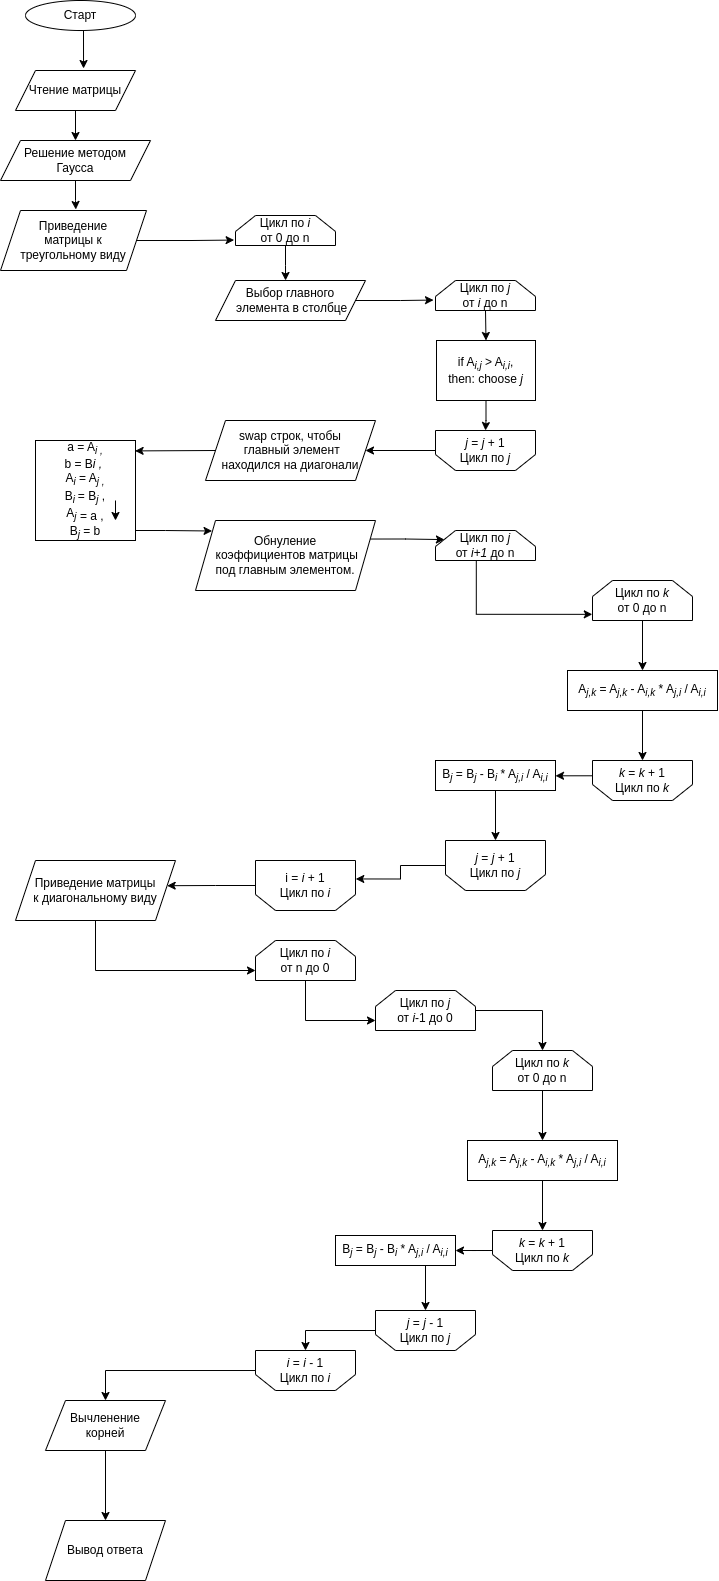
\includegraphics[scale=0.3]{img/блок-схема}
\end{figure}
\newpage
\thispagestyle{empty}
\BgThispage


\section{Listing реализованного численного метода}
\tiny
\begin{verbatim}
    void toTriangleForm() throws MatrixCreateException {
        double[][] A = matrix.getA();
        double[] B = matrix.getB();
        int n = matrix.getSize();
        for (int i = 0; i < n; i++) {
            replaceLinesInMatrix(A, B, i, chooseMainEl(A, i));
            for (int j = i + 1; j < n; j++) {
                lineSub(A, B, i, j);
            }
        }
        this.matrix = new Matrix(A, B, n);
        this.myMatrixIsTriangle = true;
    }

    void fromTriangleToDiag() throws MatrixCreateException {
        double[][] A = matrix.getA();
        double[] B = matrix.getB();
        for (int i = matrix.getSize() - 1; i >= 0; i--) {
            for (int j = i - 1; j >= 0; j--) {
                lineSub(A, B, i, j);
            }
        }
        matrix = new Matrix(A, B, matrix.getSize());
        this.myMatrixIsDiagonal = true;
    }

    double[] calculateSolutionsFromDiag() throws TryCalculateNotDIagMatrixException {
        if (myMatrixIsDiagonal) {
            double[][] A = matrix.getA();
            double[] B = matrix.getB();
            double[] solutions = new double[matrix.getSize()];
            for (int i = 0; i < matrix.getSize(); i++) {
                solutions[i] = B[i] / A[i][i];
            }
            return solutions;
        } else {
            throw new TryCalculateNotDIagMatrixException();
        }
    }

    private void lineSub(double[][] A, double[] B, int i, int j) {
        if (A[i][i] == 0) return;
        double m = A[j][i]/A[i][i];
        for (int k = 0; k < A.length; k++) {
            A[j][k] -= DoubleRounder.roundDoubleForMatrix(A[i][k] * m);
        }
        B[j] -= DoubleRounder.roundDoubleForMatrix(B[i] * m);
    }

    private void replaceLinesInMatrix(double[][] A, double[] B, int n1, int n2) {
        double b = B[n1];
        double[] a = A[n1];
        B[n1] = B[n2];
        B[n1] = b;
        A[n1] = A[n2];
        A[n2] = a;
    }

    private int chooseMainEl(double[][] A, int j) {
        int numberOfMainElLine = j;
        double maxEl = A[j][j];
        for (int i = j; i < A.length; i++) {
            if (A[i][j] > maxEl) {
                maxEl = A[i][j];
                numberOfMainElLine = i;
            }
        }
        return numberOfMainElLine;
    }
}
\end{verbatim}
\normalsize
\newpage
\thispagestyle{empty}
\BgThispage


\section{Examples}
\tiny
\begin{verbatim}
Enter the coefficients of the equation? (otherwise will be generated automatically) Y/N: Y
Enter the dimensionality of the matrix: 5
Enter the coefficients of matrices A and B line by line, separating them with a space:
0 0 0 0 0 1
0 0 0 0 0 2
0 0 0 0 0 3
0 0 0 0 0 4
0 0 0 0 0 5
Input completed.
Triangled matrix:
		0.0 0.0 0.0 0.0 0.0 | 1.0
		0.0 0.0 0.0 0.0 0.0 | 2.0
		0.0 0.0 0.0 0.0 0.0 | 3.0
		0.0 0.0 0.0 0.0 0.0 | 4.0
		0.0 0.0 0.0 0.0 0.0 | 5.0

This matrix has no solutions!
\end{verbatim}
\normalsize
Вывод верен - матрица действительно не имеет решений\\
\tiny
\begin{verbatim}
Enter the coefficients of the equation? (otherwise will be generated automatically) Y/N: Y
Enter the dimensionality of the matrix: 5
Enter the coefficients of matrices A and B line by line, separating them with a space:
1 1 1 1 1 1
1 1 1 1 1 2
1 1 1 1 1 3
1 1 1 1 1 4
1 1 1 1 1 5
Input completed.
Triangled matrix:
        1.0 1.0 1.0 1.0 1.0 | 1.0
		0.0 0.0 0.0 0.0 0.0 | 1.0
		0.0 0.0 0.0 0.0 0.0 | 2.0
		0.0 0.0 0.0 0.0 0.0 | 3.0
		0.0 0.0 0.0 0.0 0.0 | 4.0

This matrix has no solutions!
\end{verbatim}
\normalsize
Вывод верен - матрица действительно не имеет решений\\
\tiny
\begin{verbatim}
Enter the coefficients of the equation? (otherwise will be generated automatically) Y/N: Y
Enter the dimensionality of the matrix: 5
5.5 2.3 6.7 5.3 4.8 4.2
5.68 5.12 9 8.56 7.432 5
3 5 3 2 1 6.23
5 0 0 4 2.1 1
1 1 1 4 5 7
Enter the coefficients of matrices A and B line by line, separating them with a space:
Input completed.
Triangled matrix:
		5.7 5.1 9.0 8.6 7.4 | 4.2
		0.0 2.3 -1.8 -2.5 -2.9 | 0.9
		0.0 -0.0 -0.5 2.6 3.8 | 5.1
		0.0 0.0 0.0 -26.6 -36.1 | -114.5
		0.0 0.0 0.0 0.0 -5.0 | 252.6

Determinant: -875.3204265714517

Residual:
		r1 = 1.4210854715202004E-14
		r2 = 0.0
		r3 = 0.0
		r4 = 0.0
		r5 = 0.0

Answer: x1 = -21.147998767605635
		x2 = 3.8429445394256843
		x3 = -16.22595944242167
		x4 = 73.4817586845628
		x5 = -50.90493298542485
\end{verbatim}
\normalsize
Детерминант, корни матрицы и невязка вычислены верно\\
\newpage
\thispagestyle{empty}
\BgThispage


\section{Вывод}
Алгоритмическая сложность: O($N^3$)
Отличие от простого Метода Гаусса - существенное уменьшение невязки, за счёт выбора главного элемента.
Различие прямых методов от итерационных:
\begin{enumerate}
    \item Итерационным методом можно как быстрее найти решение, так и дольше - выше разброс, в то время, как прямой метод выполняется за определённое число итераций.
    \item На больших матрицах у итерационных методов ниже погрешность и не накапливаются ошибки, в отличие от прямых.
\end{enumerate}
